\section{Discussion}

We now discuss the model for the photoionization and recombination process. 

\subsection{PhotoIonization Process}

\begin{enumerate}
\item KOH + $h\nu$ \rightarrow K* + OH
\item K* + M \rightarrow K+ + e- + M
\end{enumerate}

Step 1 is the well-known phenomenon of laser-induced fluoresce in Alkali compounds (hydroxides, chlorides, etc.) which has been used to measure the species concentration of these alkali compounds in flames.[Oldenbork 1986] The excited states of the alkali compounds are weakly bound and dissociate. For KOH, there is a UV absorption band with a peak near the 248 nm wavelength of our laser, and the dissociated state creates a K atom in the excited 2P0 state [Oldenbork and Leffler 2017]. This excited K atom is known to rapidly photo luminesce. We observe this photoluminescence in our ICCD camera measurements (see Figure S\ref*{fig:SI_536_iccd}) which is on the order of our laser pulse width (10ns). The radiative lifetime of an isolated 2P0 state K atom is about 25 ns, but this lifetime will be reduced by collisional quenching, consistent with our measurements. [leffler 2017, (Smirinov (Fund. Of Ionized Gases - Table 2.8)]. 

The photodiode signal presented in Figure\ref{fig:kwt_ionization}B also is a similar measure of the KOH chemiluminescence and is observed to scale with the nominal potassium concentration. The $\Delta AS_{max}$ also shown in Figure\ref{fig:kwt_ionization}B is observed to scale with the nominal potassium concentration. Assuming that $\Delta AS_{max}$ is related to the laser-induced free electron population, this observation is evidence for a laser-induced ionization process that occurs in addition to the laser-induced chemiluminescence proposed in step 2. 

It is possible that K atoms are directly ionized in this process. However, the UV absorption cross section of K is much smaller than KOH, and the UV absorption cross section of KOH is much larger than other major species present including K (see SI). Additionally, the AS signal linearly increases with the nominal potassium concentration, even though the atomic potassium density measurements at the goldilocks region decrease with nominal potassium mass fraction (\ref{fig:kwt_ionization}A). However, the predicted KOH concentration at the goldilocks zone from CFD scales linearly with the nominal Kwt along with the PD and $\Delta AS_{max}$ signals. As mentioned previously and shown in Figure \ref{fig:kwt_ionization}A, this KOH concentration is nearly equal to the measured K concentration at the barrel exit, implying that most atomic K has become bound in KOH by the time it reaches the goldilocks region.

Together, this evidence suggests an ionization process that is related to the KOH chemiluminescence process, and not the atomic potassium. In this step the excited K atom might be ionized by a collision with a third body.  From Alkemade et al. we know that the K +M \rightarrow K+ + e- +M depends on a collision with a third body, and appears to be dependent on the potassium atom being in an excited state (known as the 'ladder model'). []It is also possible that the excited K atom is ionized by additional UV photons. The UV cross section of K is much smaller than KOH, but it is possible that the 2P0 state of K has a much higher UV cross section (see SI). 

The $\Delta AS_{max}$ signal also is observed to peak downstream of the barrel exit. A small peak in a similar location is observed in the CFD KOH concentration, but generally the centerline CFD-predicted KOH concentration is weakly dependent on position and not sufficient to explain the peak in the $\Delta AS_{max}$ signal. We do observe from the ICCD camera images for different positions that the extent of the chemiluminescence is smaller near the barrel exit and mirrors the KOH spreading. We suspect that the change in microwave transmission is related the physical size of the laser-jet interaction and could explain the peak in $\Delta AS$ signal. In this work, we do not model the transmission of microwaves between the two horns, and further work is planned to account for this effect.

\subsection{Recombination Process}

After ionization, the excited electron population decays back to equilibrium through a recombination process. We propose: 

\begin{enumerate}
\item e- + O2 + M \rightarrow O2- + M (Low Power)
\item e- + K+ + M \rightarrow K- + M (High Power)
\end{enumerate}

Finally, in step 3 the excited free electron is captured by an oxygen molecule. For high excitation densities or near the barrel exit other species can capture the electron. TODO: how to present? 

\begin{outline}
    
\1 Evidence for e- + O2 \rightarrow O2-
    \2 the decay time predicted for oxygen capture is the closest to the measured decay time. There is a significant uncertainty in the recombination coefficient for this process and our values fall within the range presented in the literature. 
    \2 The decay time appears to be independent of the position along the free jet. The decay time is difficult to quantify outside of the goldilocks region due to the AS fluctuations, but the AS magnitude is still appreciable after a few microseconds regardless of position. a similar order of magnitude to the exponential fit time constants obtained in the goldilocks region. CFD simulations (SI) show that the oxygen concentration is relatively constant along the free jet. This constant oxygen concentration of ~20\% occurs from running fuel lean, and air entrainment. 
    \2 Related, we have observed dependence of decay time on equivalence ratio (SI). However, similar to the position dependence, quantification of the decay time is difficult due to the AS fluctuations. Additionally, the profile of the torch changes with equivalence ratio (extends for high equivalence ratio), so it is difficult to deconvolve the effects of the profile change from the effects of the equivalence ratio.
\end{outline}



\subsection{Viability Analysis}

With the developed understanding of the photoionization and recombination process, we performed an assessment of the viability of the photoionization process to produce a net return in energy in seeded oxy-fuel combustion products. The methods are described in detail in the SI. Briefly, the modeling is performed with 0D chemical equilibrium calculations to determine the composition and thermophysical properties of a seeded oxy-kerosene combustion products at various temperatures and pressures, approximating various locations in a MHD generator. We then apply a nonequilibrium ionization model to determine the change in electrical conductivity due to photoionization. We then calculate the MHD power output for various photoionization power inputs and determine the regimes in which photoionization is a net energy return. We calculate a figure of merit for the photoionization process, $\gamma$, which is the ratio of the change in MHD power output, $dP_{MHD}$ for an intestinal amount of photoionization power input, $dP_{in}$. 


\begin{equation}
\gamma = \frac{dP_{MHD}}{dP_{in}} \Big|_{P_{in}=0}
\end{equation}

Therefore, a $\gamma > 1$ indicates a net energy return. For the MHD power output, we use the ideal power density in a MHD generator, given by \ref{eq:mhd_ideal_power}. (how much of SI to reproduce here?)

Figure \ref{fig:viability_gamma}A shows $\gamma$ for various temperatures and pressures.  For $\gamma > 1$ at low temperatures and pressures (blue region), the photoionization process exhibits a net energy return and is viable. For $\gamma < 1$, at high temperatures and pressures (red region) the photoionization process is not viable. The line $\gamma = 1$ is the boundary between these two regions and is defined as the 'viability line'. To determine the viability line (green dashed  line), we interpolate $\gamma$ each temperature to determine the pressure at which $\gamma = 1$. 

In Figure \ref{fig:viability_gamma}B, we show the viability lines for some different analysis conditions. TODO: finish when final plot parameters are decided. 

\begin{itemize}
    \item $\eta$ - the photoionization efficiency is the fraction of the photoionization power input that is converted to ionized electrons (ionization potential per electron). Perfect efficiency ($eta_{perf} = 1$), and an efficiency determined by the fraction of UV light absorbed by the KOH ($eta_{PI}$) are shown.
    \item The fraction of targeted volume compared to the bulk flow ($l_{bk}$). This parameter is relevant for analyzing boundary layer enhancement. for low $l_{bk}$, the photoionization power input is applied to a small volume of the flow, and for high $l_{bk}$ the photoionization power input is applied to the entire flow. see SI (TODO)
    \item Equivalence ratio. The equivalence ratio changes the oxygen molecule concentration compared to other capturing species
\end{itemize}


In Figure S\ref{fig:SI_P_zero_rxn_component} we examine viability lines considering only one reaction partner (e.g. only O2, only K+, etc.) to determine the effect of each reaction on the shape of the viability line. We observe that for temperatures below about 2000K, O2 is the dominant recombination partner for fuel lean mixtures and K+ is the dominant recombination partner for fuel rich mixtures. For higher temperatures, the temperature dependence of the H2O reaction causes it to dominate the recombination process, though recombination by K+ is still significant. Figure S\ref{fig:SI_krm_cfd_pos} shows the predicted lifetimes from different species for different axial position in the free jet and predicts that H2O and K+ overtake O2 as the dominant recombination partner at the higher temperatures closer to the barrel exit. However, as mentioned previously, the SFR closer to the barrel exit is too high to accurately measure the decay time and validate these predictions. Further work is needed to develop a better understanding of the recombination process at these high temperatures.  


\begin{figure}[h]
    \centering
    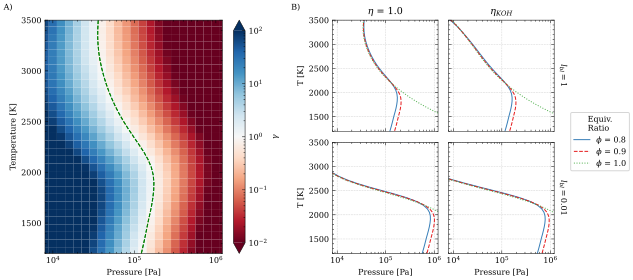
\includegraphics[width=\linewidth]{\repodir/final/figures/output/Fig7_Viability.png} 
    \caption{Figure of merit for photoionization for various temperatures and pressures. The plot is for 1\% K mass fraction, 0.8 equivalence ratio. For all analysis we assume a velocity of  The lines represent where $\gamma = 1$ for various temperatures and pressures as described in the text.}   
    \label{fig:viability_gamma}
\end{figure}



\section{Conclusion}

In conclusion, we have presented experimental evidence of UV photoionization in a potassium seeded high-velocity oxy-fuel flame. The experimental results suggest and ionization mechanism of excimer-induced KOH dissociation, followed by thermal ionization of the excited K atom. For the recombination process, we have observe a first-order recombination process that is consistent with the capture of free electrons by oxygen molecules. Using these results, we have developed a model for the photoionization and recombination process and determined the viability of the photoionization process to produce a net return in energy in seeded oxy-fuel combustion products. 